\chapter{Description of Experiments}

This chapter summarizes the range of experiments used in the current evaluation for the CFAST model. This study focused on the predicted results of the CFAST fire model and did not include an assessment of the user interface for the model.  However, all input files used for the simulations were prepared using the GUI and reviewed for correctness prior to the simulations.  The comparisons between the experiments and model predictions were characterized as semi-blind calculations, i.e., the modelers were given detailed descriptions of the test conditions, test geometry, and fire source, but did not modify model inputs from these given conditions to improve model predictions.  As such, the comparisons in this report provide an assessment of the predictive capability of the model, but not an assessment of the ability of different modelers to develop appropriate model inputs.

\section{NBS Single Room Tests with Furniture}

These data describe a series of room fire tests using upholstered furniture items in a room of fixed size but with varying opening sizes and shapes \cite{Valid:Babrauskas_Flashover}. It was selected for its well characterized and realistic fuel sources in a simple single-room geometry. In addition, the wide variation in opening size should provide challenges for current zone fire models. Peak fire size was about 2.9 MW with a total room volume of 21 m$^3$. A series of four single-room fire tests were conducted using upholstered furniture items for comparison with their free burning behavior, previously determined in a furniture calorimeter.  The experiments were conducted in a single room enclosure; ventilation to the room was provided by window openings of  varying sizes. The room was equipped with an instrumented exhaust collection system outside the window opening.  

A second similar test series also utilized was a single-room fire test using furniture as the fire source \cite{Lee:1985}. It expanded upon that data set by adding the phenomenon of wall burning. Peak fire size was about 7 MW. The room size was similar to the first test series. Figure \ref{fig:NBSFurniture} illustrates the configuration for the two test series.

\begin{figure}[\figoptions{b}]
\begin{center}
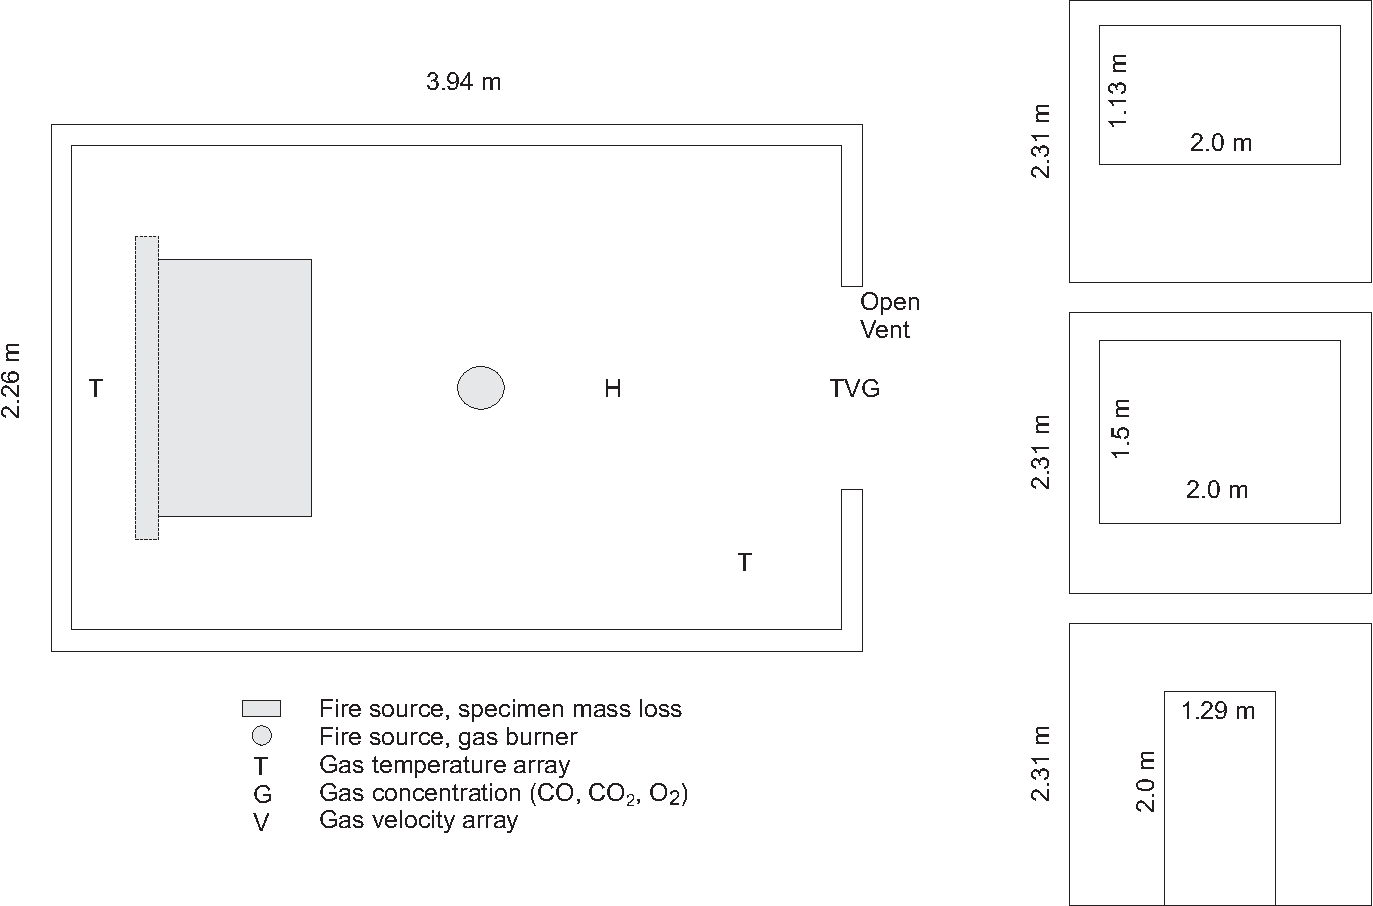
\includegraphics[width=5.0in]{FIGURES/NBS/NBSFurniture}\\
\end{center}
\caption[Plan and elevation view schematic of experimental room for NBS single room tests with furniture.]{Plan and elevation view schematic of experimental room for NBS single room tests with furniture. Note dotted lines on burning specimen indicates vertical surface for wall burning experiments.  Specimen and instrumentation placement are approximate.}
 \label{fig:NBSFurniture}
\end{figure}

The test furniture included a 28.3 kg armchair or a similar 40.0 kg love seat for the first test series. Both were of conventional wood frame construction and used polyurethane foam padding, made to minimum California State flammability requirements, and polyolefin fabric. A single piece of test furniture and igniting wastebasket were the only combustibles in the test room. 

For the second test series, room furnishings consisted of a 1.37 m wide x 1.91 m long x 0.53 m high double bed, a 2.39 X 0.89 m high headboard, and 0.51 m wide x 0.41 m deep x 0.63 m high night table. Both headboard and night table were fabricated from 12.7 mm thick plywood. The bedding was comprised of two pillows, two pillow cases, two sheets, and one blanket. The pillows had a polypropylene fabric with a polyester filling. The pillow cases and sheets were polyester-cotton. The blanket was acrylic material. The bedding was left in a "slept in" condition which was duplicated to the degree possible in each test. In all of the tests, the fire was started with match flame ignition of a 0.34 kg (240 x 140 x 240 mm high) wastebasket, filled with 0.41 kg of trash, positioned adjacent to the bed.

\section{VTT Large Hall Tests}

The experiments are described in reference~\cite{Hostikka:2001}. The series consisted three unique fire scenarios with replications for a total of 8 experiments. The experiments were undertaken to study the movement of smoke in a large hall with a sloped ceiling. The tests were conducted inside the VTT Fire Test Hall, with dimensions of 19 m high by 27 m long by 14 m wide. Figure \ref{fig:VTT_cutaway} shows the important features of the test hall. Figure \ref{fig:VTT_Schematic} shows detailed plan, side and perspective schematic diagrams of the experimental arrangement. Each test involved a single heptane pool fire, ranging from 2~MW to 4~MW. Figure \ref{fig:VTT_2MW_fire} is a photo of a 2~MW fire. Four types of measurements were used in the present evaluation -- the hot gas layer temperature and depth, average flame height and the plume temperature. Three vertical arrays of thermocouples, plus two thermocouples in the plume, were compared to model simulation results. The hot gas layer temperature and height were reduced from an average of the three thermocouple arrays using a standard algorithm. The ceiling jet temperature was not considered, because the ceiling in the test hall is not flat, and the model algorithm is not appropriate for these conditions.

\begin{figure}[\figoptions{b}]
\begin{center}
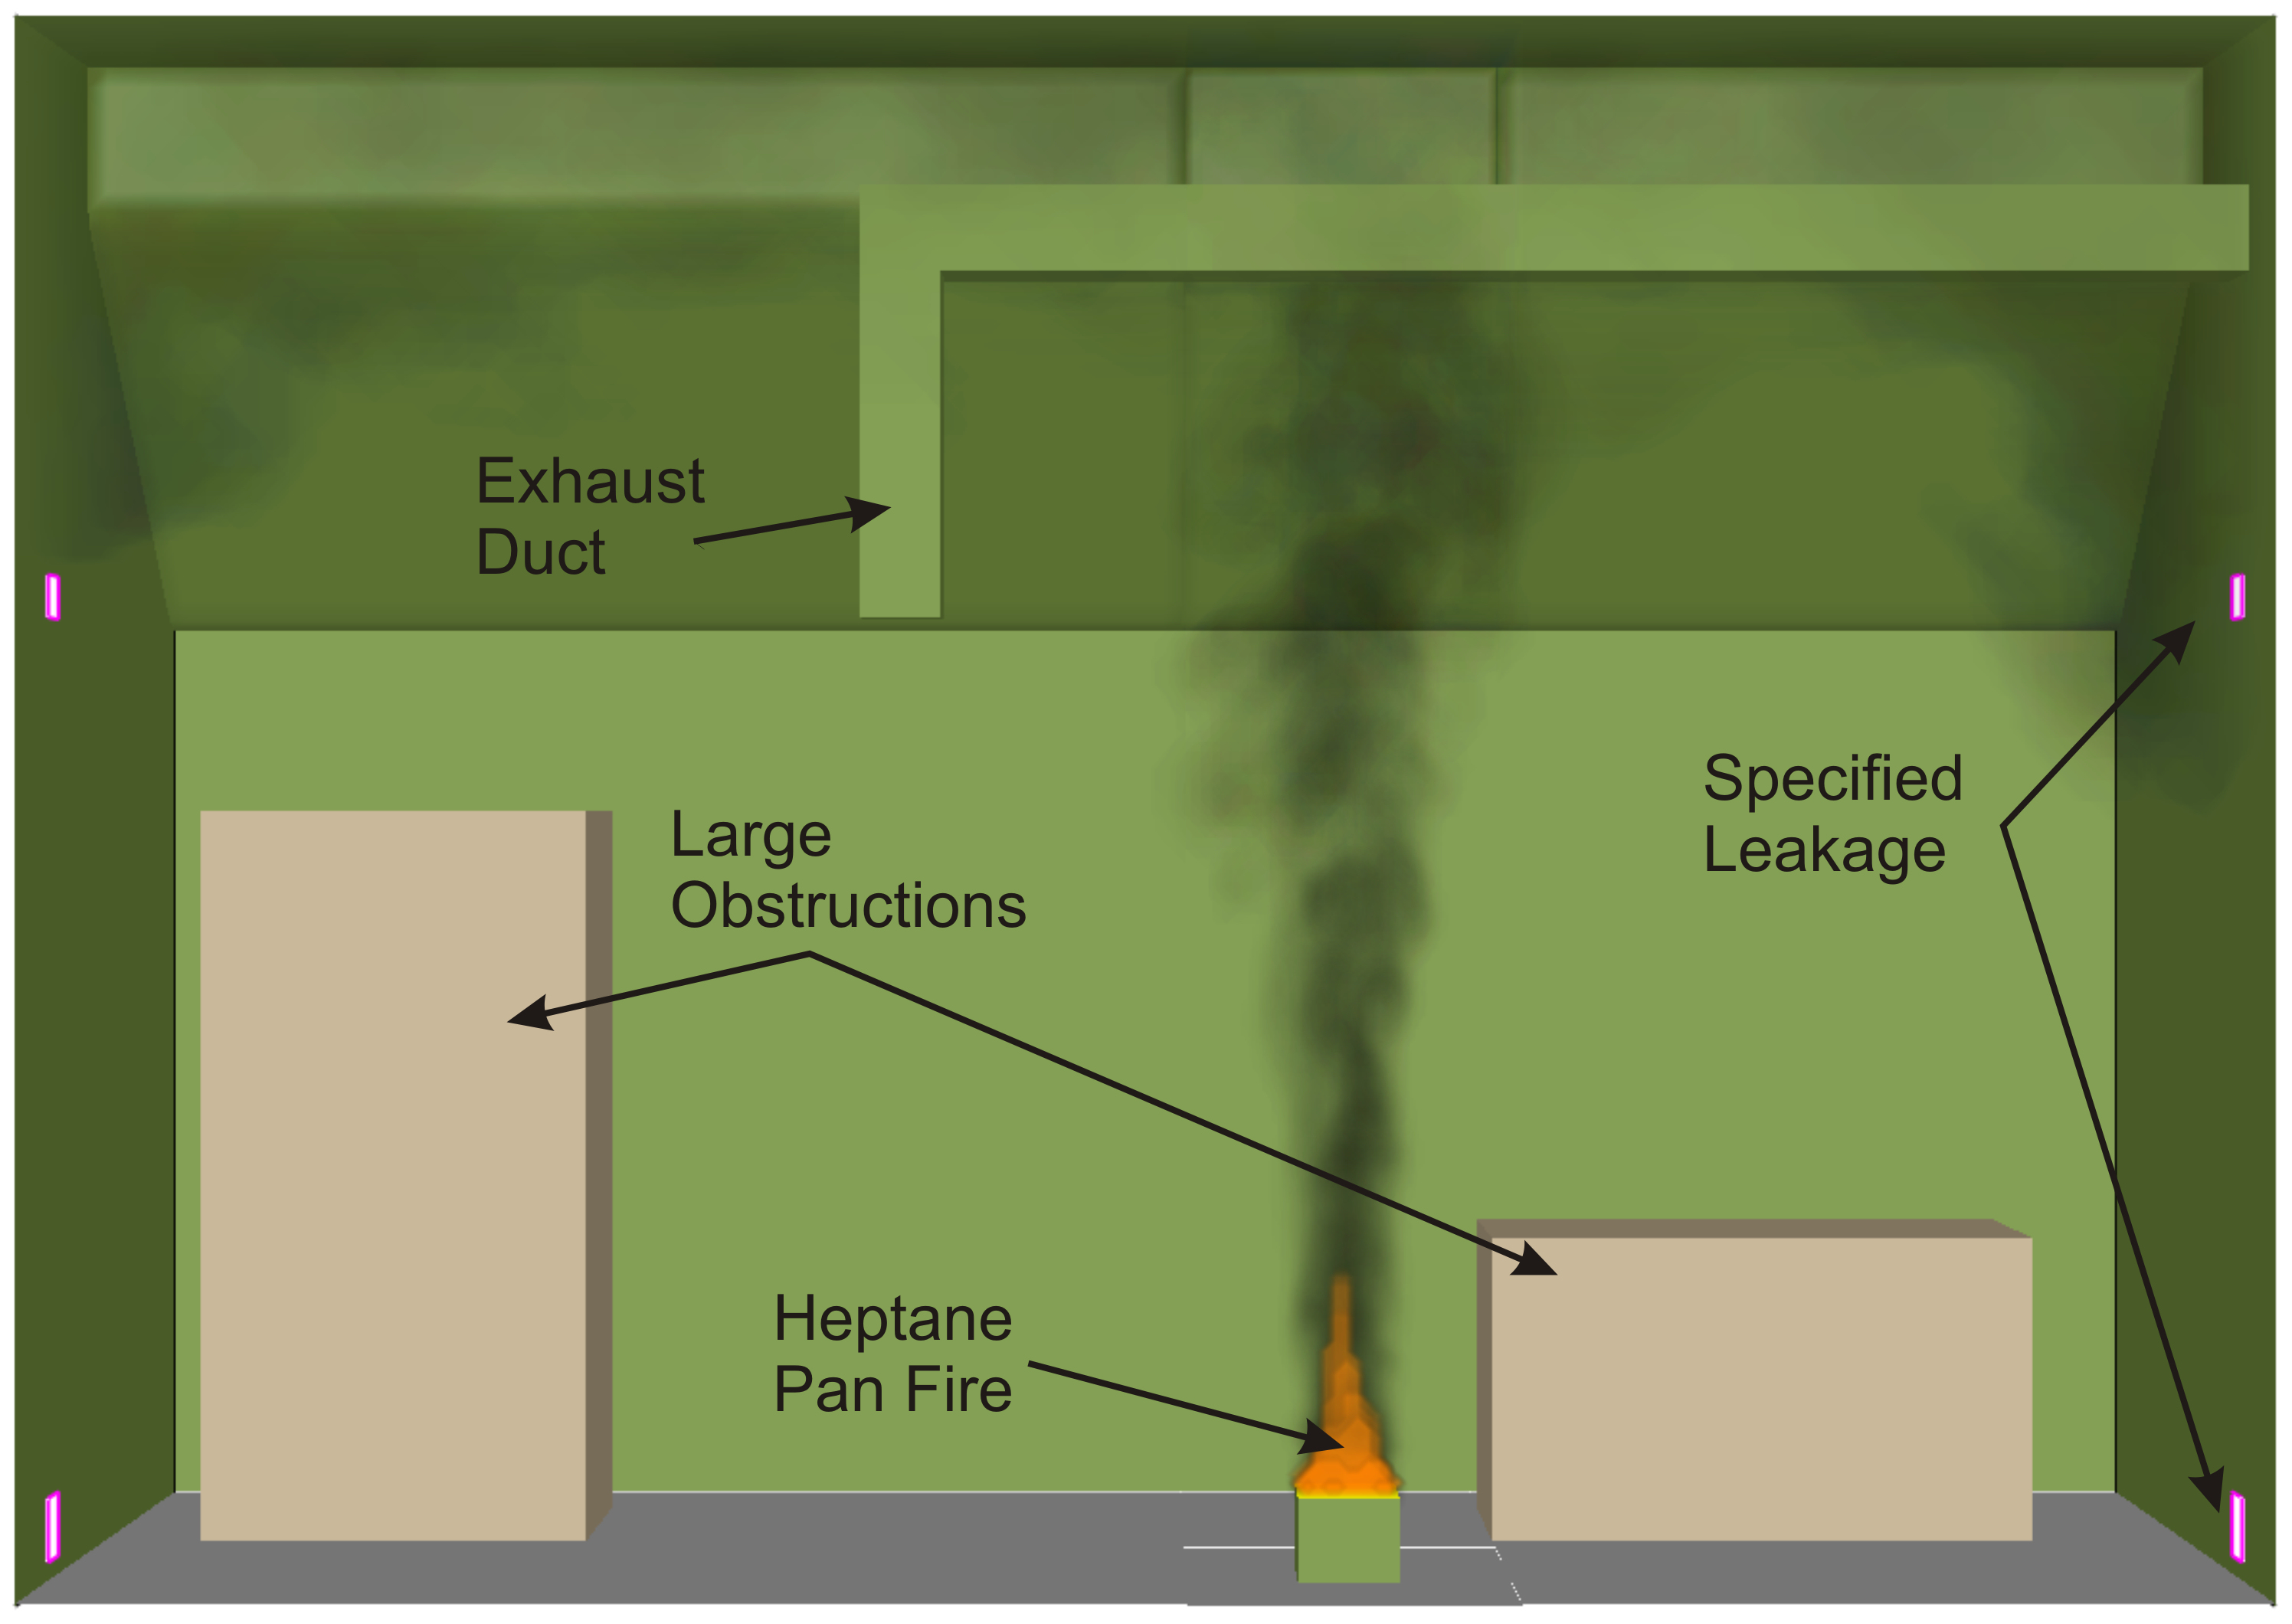
\includegraphics[width=5.0in]{FIGURES/VTT/VTT_Cut_Away}\\
\end{center}
\caption{Cut-Away View of Case 2 of the VTT Large Hall Tests.}
 \label{fig:VTT_cutaway}
\end{figure}

\begin{figure}[\figoptions{b}]
\begin{center}
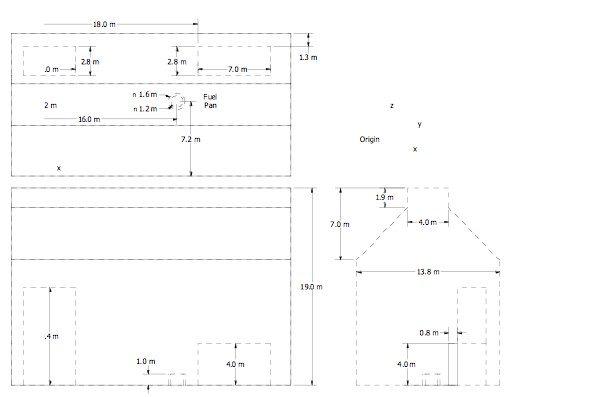
\includegraphics[width=8.0in, angle=90]{FIGURES/VTT/VTT_Schematic}\\
\end{center}
\caption{Plan, side and perspective schematic drawings of the experimental arrangement of the VTT large hall fire tests, including the fuel pan}
 \label{fig:VTT_Schematic}
\end{figure}

\begin{figure}[\figoptions{b}]
\begin{center}
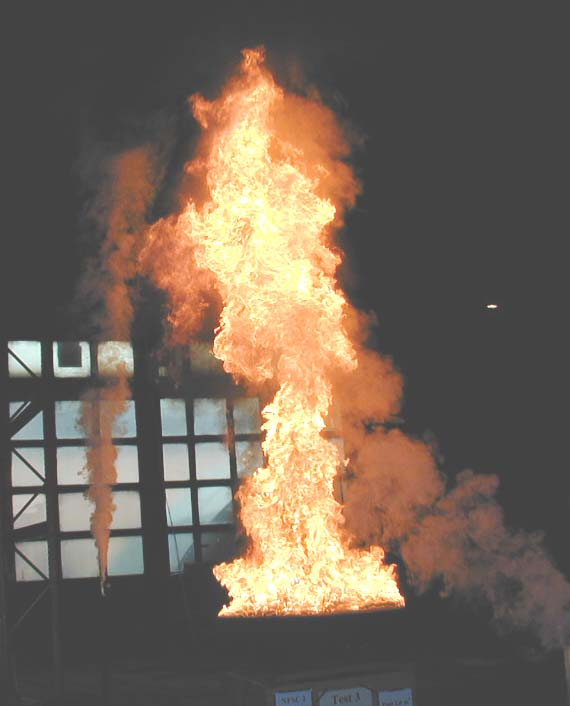
\includegraphics[width=3.0in]{FIGURES/VTT/VTT_2MW_fire}\\
\end{center}
\caption{Photo of a 2 MW heptane fire during the VTT large hall tests. Photo provided by Simo Hostikka, VTT.}
 \label{fig:VTT_2MW_fire}
\end{figure}

The VTT test report lacks some information needed to model the experiments, so some information was based on private communications with the principal investigator, Simo Hostikka. Details used to conduct the model simulations is presented in reference \cite{NRCNUREG1824Experimental}, including information on the fire, the compartment, and the ventilation.

The walls and ceiling of the test hall consist of a 1 mm thick layer of sheet metal on top of a 5 cm layer of mineral wool. The floor was constructed of concrete. The report does not provide thermal properties of these materials. Thermophysical properties of the materials that were used in the simulations are given in table \ref{tab:VTT_Thermals}.

\begin{table}[h!]
\begin{center}
\caption{Thermophysical Properties for VTT Large Hall Tests}
\label{tab:VTT_Thermals}
\vspace{0.1in}
\begin{tabular}{|l|c|c|c|c|c|}
\hline
Material & Conductivity & Specific Heat & Density & Thickness & Emissivity\\
 & W/m$^{\circ}$C & J/kg$^{\circ}$C & kg/m$^3$ & m & \\ \hline
\hline
Steel ICFMP BE2 & 54 &        425 &       7850 &      0.001 &       0.95  \\ \hline
Concrete ICFMP BE2 &          2 &        900 &        230 &       0.15 &       0.95 \\ \hline
\end{tabular}  
\end{center}
\end{table}

In Cases 1 and 2, all doors were closed, and ventilation was restricted to leakage through the building envelope. Precise information on air infiltration during these tests is not available. The scientists who conducted the experiments recommend a leakage area of about 2~m$^2$, distributed uniformly throughout the enclosure. By contrast, in Case 3, the doors located in each end wall (Doors 1 and 2, respectively) were open to the external ambient environment. These doors are each 0.8 m wide by 4 m high, and are located such that their centers are 9.3 m from the south wall. The test hall had a single mechanical exhaust duct, located in the roof space, running along the center of the building. This duct had a circular section with a diameter of 1 m, and opened horizontally to the hall at a distance of 12 m from the floor and 10.5 m from the west wall. Mechanical exhaust ventilation was operational for Case 3, with a constant volume flow rate of 11 m$^3$/s drawn through the 1 m diameter exhaust duct. 

Each test used a single fire source with its center located 16 m (52 ft) from the west wall and 7.4 m from the south wall. For all tests, the fuel was heptane in a circular steel pan that was partially filled with water. The pan had a diameter of 1.17 m for Case 1 and 1.6 m for Cases 2 and 3. In each case, the fuel surface was 1 m above the floor. The trays were placed on load cells, and the HRR was calculated from the mass loss rate. For the three cases, the fuel mass loss rate was averaged from individual replicate tests. In the HRR estimation, the heat of combustion (taken as 44.6 kJ/g) and the combustion efficiency for n-heptane was used.  In this report, a combustion efficiency of 0.85 $\pm$ 0.12 (or $\pm$ 14 \%) was used for the VTT pool fire tests \cite{NRCNUREG1824Experimental}. Due to the relatively large value of the uncertainty associated with the combustion efficiency the uncertainty in HRR is dominated by the uncertainty in the combustion efficiency. Uncertainty in the mass loss rate measurement also contributed to the overall uncertainty, and the uncertainty in HRR was estimated as 15 \% \cite{NRCNUREG1824Experimental}. Figure \ref{fig:VTT_HRR} show the prescribed HRR as a function of time during Cases 1 to 3, respectively. The radiative fraction was assigned a value of 0.35 \cite{NRCNUREG1824Experimental}, similar to many smoky hydrocarbons \cite{Hamins:1991}. The relative combined expanded (2$\sigma$) uncertainty in this parameter was assigned a value of $\pm$ 20 \%, which is typical of uncertainty values reported in the literature for this parameter. Further details of the model inputs used for these simulations are included in reference \cite{NRCNUREG1824Experimental}.

\begin{figure}[p]
\begin{center}
\begin{tabular}{c}
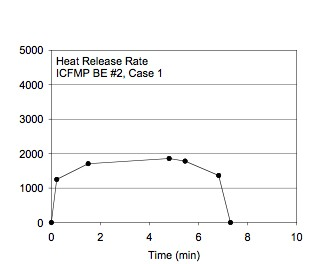
\includegraphics[width=2.6in]{FIGURES/VTT/VTT_Case1_HRR} \\
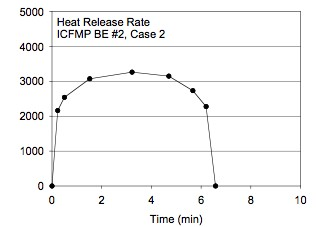
\includegraphics[width=2.6in]{FIGURES/VTT/VTT_Case2_HRR} \\
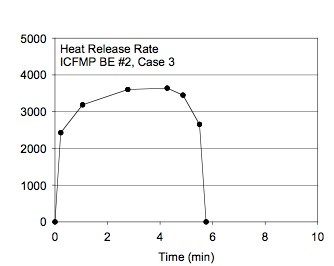
\includegraphics[width=2.6in]{FIGURES/VTT//VTT_Case3_HRR}
\end{tabular}
\end{center}
\caption{Prescribed Heat Release Rate as a Function of Time for VTT Large Hall Tests.} \label{fig:VTT_HRR}
\end{figure}

\section{NIST/NRC Test Series}

These experiments, sponsored by the US NRC and conducted at NIST, consisted of 15 large-scale experiments performed in June 2003. All 15 tests were included in the validation study. The experiments are documented in Ref.~\cite{Hamins:2005}. The fire sizes ranged from 350 kW to 2.2 MW in a compartment with dimensions 21.7~m by 7.1~m by 3.8~m high, designed to represent a compartment in a nuclear power plant containing power and control cables. A photo of the fire seen through the compartment doorway is shown in figure \ref{fig:NISTNRC_1MW_fire}. Figure \ref{fig:NISTNRC_Summary} shows the important features of the test hall. Figure \ref{fig:NISTNRC_Detailed} shows detailed plan, side and perspective schematic diagrams of the experimental arrangement. The walls and ceiling were covered with two layers of marinate boards, each layer 0.0125~m thick. The floor was covered with one layer of gypsum board on top of a layer of plywood. Thermo-physical and optical properties of the marinate and other materials used in the compartment are given in reference \cite{Hamins:2005}. The room had one door and a mechanical air injection and extraction system. Ventilation conditions, the fire size, and fire location were varied. Numerous measurements (approximately 350 per test) were made including gas and surface temperatures, heat fluxes and gas velocities. Detailed schematic diagrams of the experimental arrangement are shown in figure \ref{fig:NISTNRC_Detailed}. Table \ref{tab:NISTNRC_Matrix} shows the experimental conditions for all 15 tests. 

\begin{figure}[\figoptions{t}]
\begin{center}
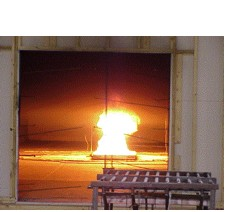
\includegraphics[width=4.0in]{FIGURES/NIST_NRC/NISTNRC_1MW_fire}\\
\end{center}
\caption{Photograph of a 1 MW heptane fire seen through the open doorway. Photo provided by Anthony Hamins, NIST.}
 \label{fig:NISTNRC_1MW_fire}
\end{figure}

\begin{figure}[\figoptions{t}]
\begin{center}
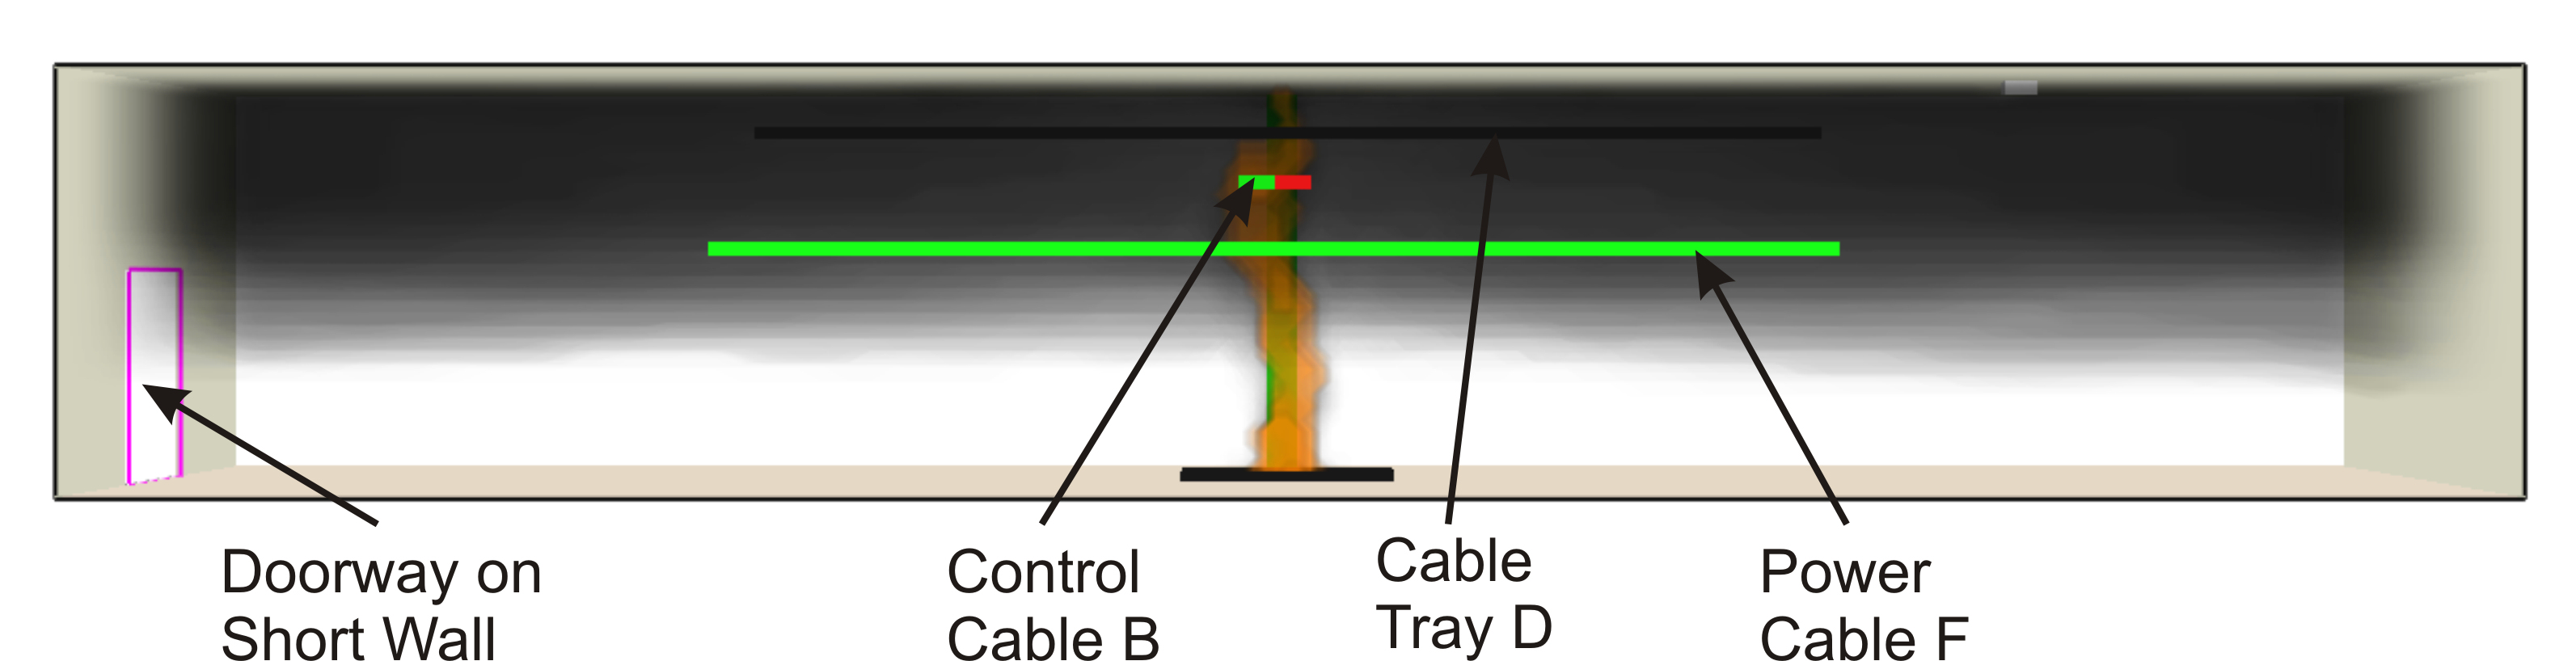
\includegraphics[width=5.0in]{FIGURES/NIST_NRC/NISTNRC_Summary}\\
\end{center}
\caption{Cross-section View of the NIST NRC Test Configuration.}
 \label{fig:NISTNRC_Summary}
\end{figure}

\begin{figure}[\figoptions{t}]
\begin{center}
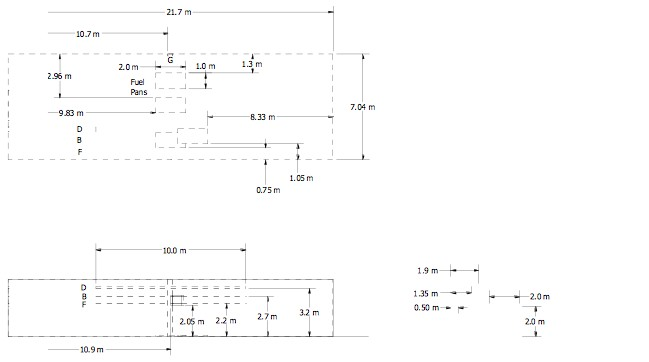
\includegraphics[width=8.0in, angle=90]{FIGURES/NIST_NRC/NISTNRC_Detailed}\\
\end{center}
\caption{Plan, side and perspective schematic drawings of the NIST NRC experimental arrangement. The fuel pan and cables B, D, F, and G (dotted lines) are also shown.}
 \label{fig:NISTNRC_Detailed}
\end{figure}

\begin{table}
\begin{center}
\caption{Test Matrix and Experimental Conditions for NIST NRC Tests}
\label{tab:NISTNRC_Matrix}
\vspace{0.1in}
\begin{tabular}{|c|c|c|c|c|c|}
\hline
Test & Nominal Peak & Cable & Fuel; Burner Location & Door & Mechanical\\
 & $\dQ$ (MW) & Type &  &  & Ventilation \\ \hline
\hline
1 & 0.35 & XPE\superscript{a} & Heptane; Center & Closed & Off \\ \hline
2 & 1 & XPE & Heptane; Center & Closed & Off \\ \hline
3 & 1 & XPE & Heptane; Center & Open & Off \\ \hline
4 & 1 & XPE & Heptane; Center & Closed & On \\ \hline
5 & 1 & XPE & Heptane; Center & Open & On \\ \hline
6 & \multicolumn{5}{|c|}{Not Conducted} \\ \hline
7 & 0.35 & PVC\superscript{b} & Heptane; Center & Closed & Off \\ \hline
8 & 1 & XPE & Heptane; Center & Closed & Off \\ \hline
9 & 1 & XPE & Heptane; Center & Open & Off \\ \hline
10 & 1 & PVC & Heptane; Center & Closed & On \\ \hline
11& \multicolumn{5}{|c|}{Not Conducted} \\ \hline
12 & \multicolumn{5}{|c|}{Not Conducted} \\ \hline
13 & 2 & XPE & Heptane; Center & Closed & Off \\ \hline
14 & 1 & XPE & Heptane; 1.8 m from N wall & Open & Off \\
 & & & on E-W centerline & & \\ \hline
15 & 1 & PVC & Heptane; 1.25 m from S wall & Open & Off \\ 
 & & & on E-W centerline & & \\ \hline
 16 & 2 & PVC & Heptane; Center & Closed & On \\ \hline
 17 & 1 & PVC & Toluene; Center & Closed & Off \\ \hline
18 & 1 & XPE & Heptane; 1.55 m from S wall & Open & Off \\
 & & & 1.50 m E of centerline & & \\ \hline 
\multicolumn{6}{l}{a - XPE cable has crosslinked polyethylene jacket insulation} \\
\multicolumn{6}{l}{b - PVC cable has a polyvinylchloride jacket insulation}
\end{tabular}  
\end{center}
\end{table}

The compartment had a 2 m by 2 m door in the middle of the west wall. Some of the tests had a closed door and no mechanical ventilation, and in those tests the measured compartment leakage was an important consideration. Reference \cite{Hamins:2005} reports leakage area based on measurements performed periodically during the test series. For the closed door tests, the leakage area used in the simulations was based on the last available measurement. It should be noted that the chronological order of the tests differed from the numerical order \cite{Hamins:2005}. 

The mechanical ventilation and exhaust was used during some test, providing about 5 air changes per hour. The supply duct was positioned on the long wall, about 2 m off the floor. An exhaust duct of equal area to the supply duct was positioned on the opposite wall at a comparable location. The flow rates through the supply and exhaust ducts were measured in detail during breaks in the testing, in the absence of a fire. During the tests, the flows were monitored with single bi-directional probes during the tests themselves.

A single nozzle was used to spray liquid hydrocarbon fuels onto a 1 m by 2 m fire pan that was about 0.02 m deep. The test plan originally called for the use of two nozzles to provide the fuel spray. Experimental observation suggested that the fire was more steady with the use of a single nozzle. In addition, it was observed that the actual extent of the liquid pool was well-approximated by a 1 m circle in the center of the pan. For safety reasons, the fuel flow was terminated when the lower-layer oxygen concentration dropped to approximately 15~\% by volume. The fuel used in 14 of the tests was heptane, while toluene was used for one test. The HRR was determined using oxygen consumption calorimetry (figure \ref{fig:NISTNRC_HRR} shows a sample heat release rate for one of the tests in the series). The recommended uncertainty values for HRR were 17~\% for all of the tests. The radiative fraction was measured in an independent study for the same fuels using the same spray burner as used in the test series \cite{Hamins:2003}. The value of the radiative fraction and its uncertainty were reported as 0.44 $\pm$ 16 \% and 0.40 $\pm$ 23 \% for heptane and toluene, respectively. Further details of the model inputs used for these simulations are included in reference \cite{NRCNUREG1824Experimental}.

\begin{figure}[\figoptions{t}]
\begin{center}
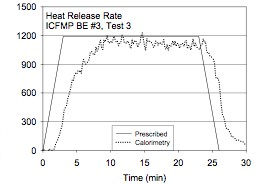
\includegraphics[width=3.0in]{FIGURES/NIST_NRC/NISTNRC_HRR}\\
\end{center}
\caption{Measured and prescribed heat release rate as a function of time during Test 3 of the NIST NRC test series}
 \label{fig:NISTNRC_HRR}
\end{figure}


\section{FM/SNL Test Series}

The Factory Mutual and Sandia National Laboratories (FM/SNL) Test Series was a series of 25 fire tests conducted in 1985 for the NRC by Factory Mutual Research Corporation (FMRC), under the direction of Sandia National Laboratories (SNL).  The primary purpose of these tests was to provide data with which to validate computer models for various types of NPP compartments.  The experiments were conducted in an enclosure measuring 18 m x 12 m x 6 m, constructed at the FMRC fire test facility in Rhode Island.  Figure \ref{fig:FMSNL_Detailed} shows detailed schematic drawings of the compartment from various perspectives.  The FM/SNL test series is described in detail, including the types and locations of measurement devices, as well as some results in References \cite{Nowlen:1987, Sandia:1989}.

\begin{figure}
\begin{center}
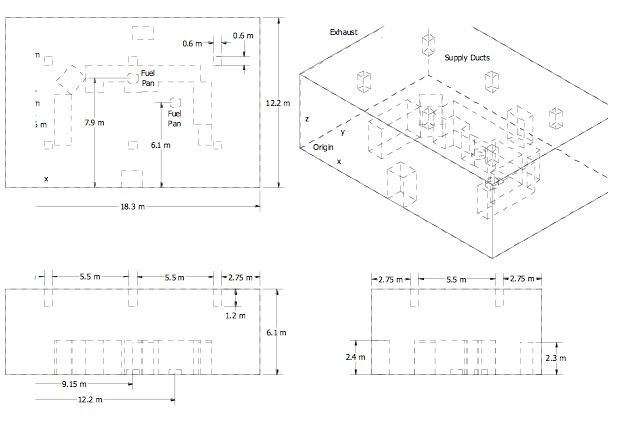
\includegraphics[width=8.0in, angle=90]{FIGURES/FM_SNL/FMSNL_Detailed}\\
\end{center}
\caption{Detailed plan, side, and perspective schematic drawings of the FM/SNL experimental arrangement, including the supply and exhaust ducts, and the fuel pan.}
 \label{fig:FMSNL_Detailed}
\end{figure}
 
All of the tests involved forced ventilation to simulate typical nuclear power plant installation practices.  Four of the tests were conducted with a full scale control room mockup in place.  Parameters varied during the experiments included fire HRR, enclosure ventilation rate, and fire location. 
 
Data from three of these experiments (Tests 4, 5, and 21) were used since these tests were documented far more completely than other tests in the series. In these tests, the fire source was a 0.91 m diameter propylene gas burner. For Tests 4 and 5, the burner was centered along the longitudinal axis centerline, 6.1 m laterally from the nearest wall, and the burner rim was located approximately 0.1 m above the floor.  For Test 21, the fire source was placed within a simulated benchboard electrical cabinet.
 
 The value of heat release rate was determined using oxygen consumption calorimetry in the exhaust stack with a correction applied for the CO$_2$ in the upper layer of the compartment.  The uncertainty of the fuel mass flow was not documented. All three tests selected for this study had the same target peak heat release rate of 516 kW.  A 4 min �t-squared� growth profile preceded the target heat release rate. The test report contains time histories of the measured  heat release rate, for which the average sustained  heat release rate following the ramp up for Tests 4, 5, and 21 have been estimated as 510 kW, 480 kW, and 470 kW, respectively.   Once reached, the peak  heat release rate was maintained essentially constant during a steady burn period of 6 min in Tests 4 and 5, and 16 min in Test 21.   Figure \ref{fig:FMSNL_HRR} shows the specified and the measured   \cite {Nowlen:1987} heat release rate as a function of time during Test 21 of the FM/SNL test series. The specified curves are used in the model calculations rather than the measured time-dependent curves, because the fuel flow was maintained a constant and fluctuations in the heat release rate are expected from calorimetry measurements.  Also, there was some concern with the quality of the heat release rate measurement as the test report notes that during Tests 4, 5, and 21 there was a downward bias in the measured  values due to �significant� loss of effluent from the exhaust hood. This bias was treated as an additional uncertainty, and the relative combined expanded uncertainty was assumed to equal $\pm$ 20 \% \cite{NRCNUREG1824Experimental}, which is somewhat larger than typical calorimetric measurement uncertainty.  The radiative fraction was not measured during the experiment, but in this study it is assumed to equal 0.35, which is typical for a smoky hydrocarbons \cite{Tewarson:1986, Tewarson:2003}.  The expanded uncertainty in this value was taken as $\pm$ 20 \% \cite{NRCNUREG1824Experimental}, a value typical of reported uncertainty \cite{Hamins:2003, Hamins:1991}.  It was further assumed that the radiative fraction was about the same in Test 21 as the other tests, as fuel burning occurred outside of the electrical cabinet in which the burner was placed.  

\begin{figure}[\figoptions{t}]
\begin{center}
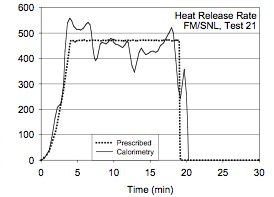
\includegraphics[width=3.0in]{FIGURES/FM_SNL/FMSNL_HRR}\\
\end{center}
\caption{Prescribed (dotted line) and measured (solid line) heat release rate as a function of time during Test 21 of the FM/SNL test series}
 \label{fig:FMSNL_HRR}
\end{figure}

Four types of measurements were conducted during the FM/SNL test series that are used in the current model evaluation study, including the HGL temperature and depth, and the ceiling jet and plume temperatures.  Aspirated thermocouples were used to make all of the temperature measurements.  Generally, aspirated thermocouple (TC) measurements are preferable to bare-bead TC measurements, as systematic radiative exchange measurement error is reduced \cite{NRCNUREG1824Experimental}.  For the relatively low temperatures observed ($<$100 $^\circ$C), however, the differences are expected to be small \cite{NRCNUREG1824Experimental}.  

Aspirated thermocouple measurements for the range of temperatures measured are typically accurate to a few degrees ($^\circ$C) \cite{NRCNUREG1824Experimental}.  The temperatures were measured using the aspirated thermocouples in Sectors 1, 2 and 3 of the compartment.  In addition, there were some near-ceiling TCs placed directly above the burner in Tests 4 and 5.  

Data from all of the vertical thermocouple trees were used when reducing the HGL height and temperature. For the FM/SNL Tests 4 and 5, Sectors 1, 2, and 3 were used, all weighted evenly \cite{NRCNUREG1824Experimental}.  For Test 21, Sectors 1 and 3 were used, evenly weighted. Sector 2 was partially within the fire plume in Test 21 and was not used in the calculation of hot gas layer temperature \cite{NRCNUREG1824Experimental}.

\section{iBMB Compartment Tests}

A series of small compartment kerosene pool fire experiments, conducted at the
Institut f�r Baustoffe, Massivbau und Brandschutz (iBMB) of Braunschweig University of
Technology in Germany in 2004 \cite{Klein-Helbetaling:2005}.  The results from Test 1 were
considered here.  These experiments involved relatively large fires in a relatively small (3.6 m x 3.6 m x 5.7 m) concrete enclosure. Figure  \ref{fig:iBMB_Pool_Detailed} shows plan, side and perspective schematic drawings
of the experimental arrangement, including the location of the fuel pan, which was located at the
center of the compartment.

\begin{figure}
\begin{center}
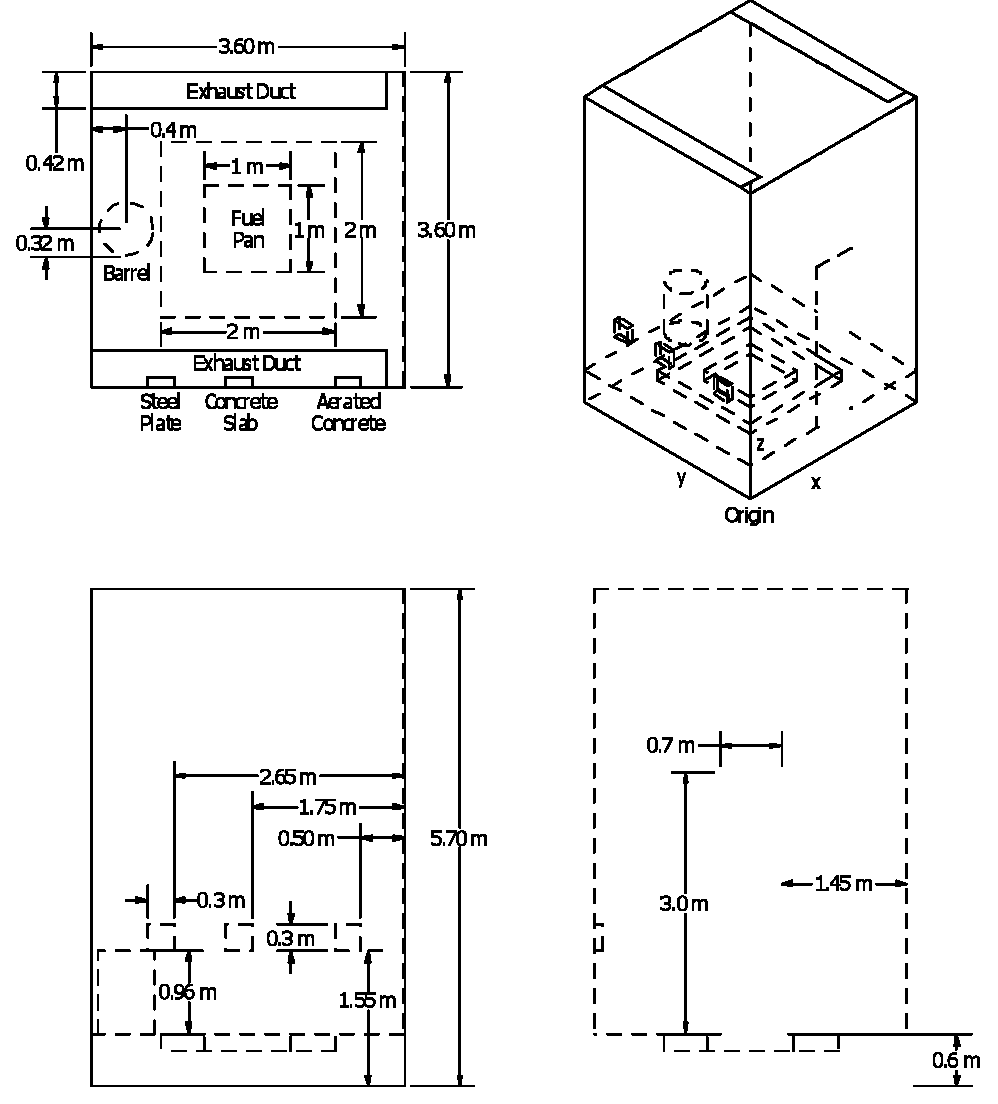
\includegraphics[width=6.5in]{FIGURES/iBMB/iBMB_Pool}\\
\end{center}
\caption{Detailed plan, side, and perspective schematic drawings of the iBMB pool fire experimental arrangement.}
 \label{fig:iBMB_Pool_Detailed}
\end{figure}
 
 Only a portion of Test 1 was selected for consideration in the present study, because a significant amount of data was lost in Test 2, and the measured ${\dQ}$  during Test 3 exhibited significant amounts of fluctuation. Five types of measurements that were conducted during the test series were used in the model evaluation reported here.  These included the HGL temperature and depth, the temperature of targets and compartment surfaces, and heat flux. In addition, figure \ref{fig:iBMB_HRR} shows the heat release rate for Test 1, which was estimated from a mass loss rate measurement.  In this calculation, the heat of combustion and the combustion efficiency were taken as 42.8 MJ/kg and 1, respectively, as suggested by Refs. \cite{NRCNUREG1824Experimental, Riese:2004}.  There were several reported difficulties in measuring the mass loss rate, including data loss due to an instrument malfunction and significant fluctuations in the measured mass loss rate. Due to these measurement issues and because the combustion efficiency was not well-characterized, the ${\dQ}$ uncertainty was assigned a relatively large expanded uncertainty of $\pm$ 25 \% \cite{NRCNUREG1824Experimental}.
 
 \begin{figure}
\begin{center}
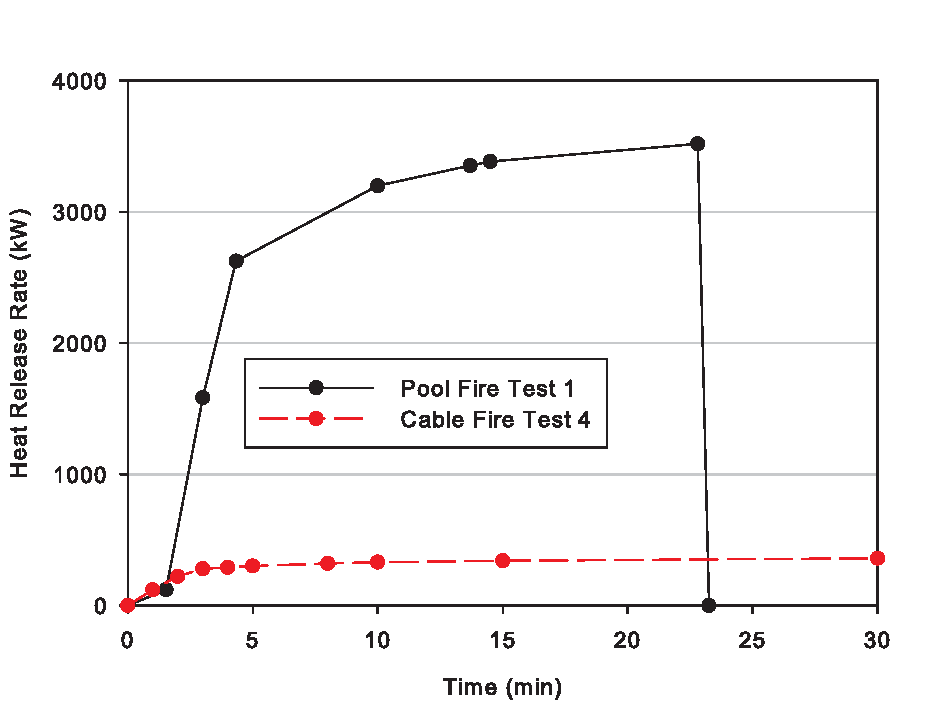
\includegraphics[width=4.0in]{FIGURES/iBMB/iBMB_HRR}\\
\end{center}
\caption{Estimated heat release rate for the iBMB fire experiments.}
 \label{fig:iBMB_HRR}
\end{figure}

A second series of fire experiments in 2004, conducted under the International Collaborative Fire Model Project (ICFMP) involved realistically routed cable
trays inside the same concrete enclosure at iBMB \cite{Riese:2004}. The compartment was configured slightly differently with a ceiling height of 5.6 m. A schematic diagram from plan, side, and perspective views of the experimental arrangement is shown in figure \ref{fig:iBMB_Cable_Detailed}. Six types of measurements conducted during the test series were used in the evaluation conducted here, including the HGL temperature and depth, oxygen gas concentration, the temperature of targets and compartment surfaces, and heat flux.

\begin{figure}
\begin{center}
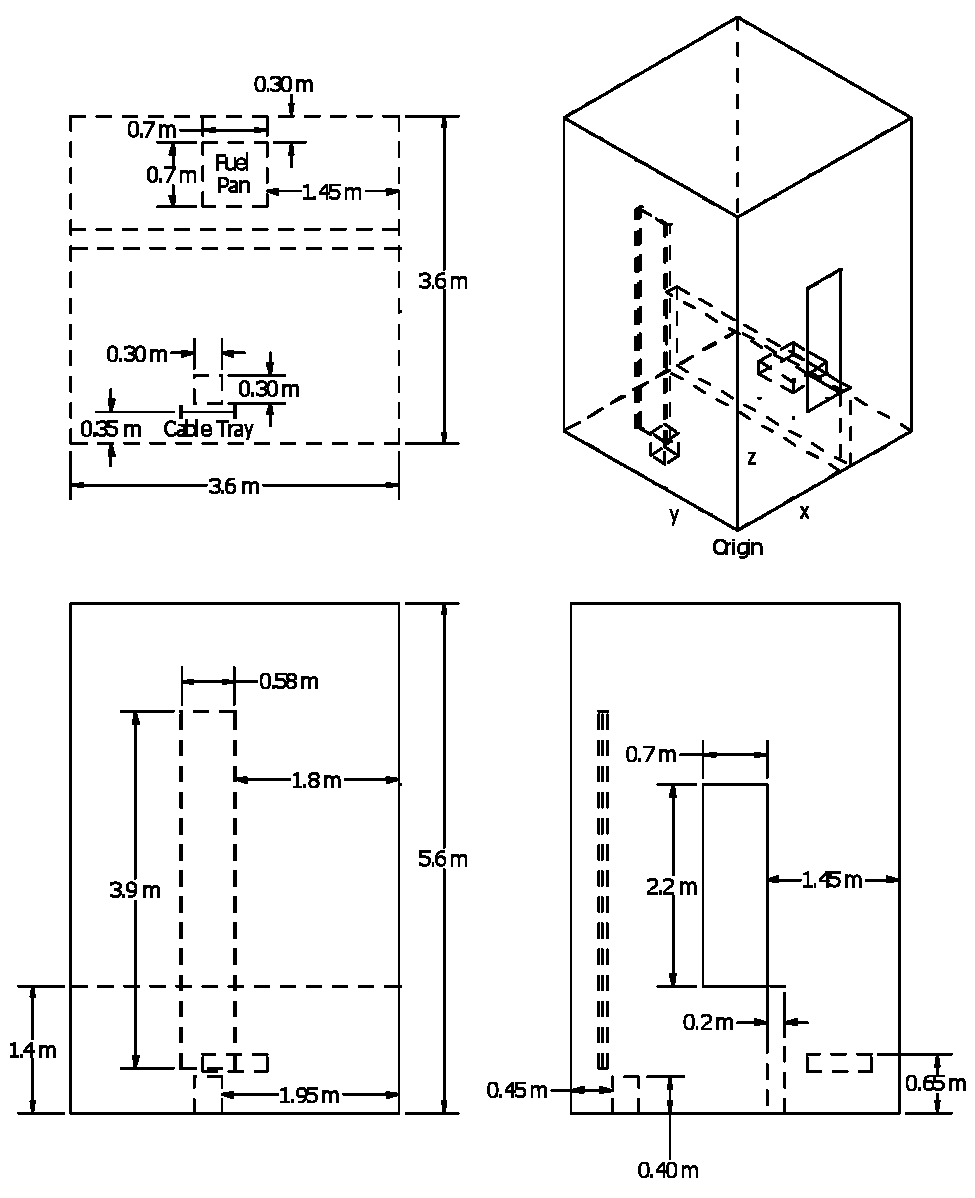
\includegraphics[width=6.5in]{FIGURES/iBMB/iBMB_Cable}\\
\end{center}
\caption{Detailed plan, side, and perspective schematic drawings of the iBMB cable fire experimental arrangement.}
 \label{fig:iBMB_Cable_Detailed}
\end{figure}

The results of four tests were
available, of which one has been used in the current study.
These tests were conducted primarily for the evaluation of cable ignition and flame spread.
The results were erratic, and no replicate experiments were performed. Given the primitive
nature of the ignition and spread algorithms within the models, it was decided that only
a qualitative analysis would be possible with the data from three of the four experiments.
However, in one experiment, the first 20 minutes involved a fairly well-characterized ethanol
pool fire burning on the opposite side of the compartment from the cable tray. This part of
the experiment has been used as part of the model evaluation.

The first part of the test consisted of preheating the cable trays in the room with a 1 m$^2$ round pan on the floor filled with ethanol (ethyl alcohol) used as the preheating source.  At 30 min, a propane gas burner was used as the fire source � this was not considered because only the first 20 min of the test was used in this validation study.  
Exhaust products were collected in an exhaust duct and the $\dQ$  was measured using the oxygen calorimetry.  For the purpose of this study, the measured $\dQ$ was used as direct input to the various fire models.  The first 20 min of data were used for the model evaluation. After 20 min, the  $\dQ$ became relatively noisy.  Figure \ref{fig:iBMB_HRR} shows the HRR. The relative combined expanded uncertainty was assigned a value of $\pm$15 \%, consistent with typical values of this parameter \cite{NRCNUREG1824Experimental}.

\section{NBS Multi-Compartment Test Series}

The National Bureau of Standards (NBS, former name of NIST) Multi-Compartment Test Series consisted of 45 fire tests representing 9 different sets of conditions were conducted in a three-room suite.  The experiments were conducted in 1985 and are described in detail in reference \cite{Peacock:1988}.  The suite consisted of two relatively small rooms, connected via a relatively long corridor. Total volume of the structure was approximately 100 m$^2$. The fire source, a gas burner, was located against the rear wall of one of the small compartments as seen in Figure \ref{fig:NBS_100kW_fire} for a 100 kW fire.  Figures \ref{fig:NBS_Summary} and \ref{fig:NBS_Detailed} presents the experimental arrangement in the form of plan, side and perspective schematic drawings of the compartments. Fire tests of 100 kW, 300 kW and 500 kW were conducted. For the current  study, three 100 kW fire experiments have been used, including Test 100A from Set 1, Test 100O from Set 2, and Test 100Z from Set 4. For the NBS Multi-room series, Tests 100A, 100O and 100Z were selected for study, because they were constructively used in a previous validation study [\cite{EPRI}, and because these tests had  the steadiest values of measured heat release rate during the steady burning period. The selected data are also available in Reference \cite{EPRI}.   Reference \cite{NRCNUREG1824Experimental} provides information used as model input for simulation of the NBS tests, including information on the compartment, the fire, the ventilation, and ambient conditions. The data in the NBS data set was acquired every 10 s with a 6 s time-average.  This time-averaging interval was somewhat smaller than all of the other experimental series, which were time-averaged over a 10 s interval. 

\begin{figure}
\begin{center}
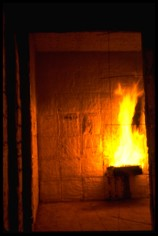
\includegraphics[width=2.0in]{FIGURES/NBS/NBS_100kW_fire}  \\
\end{center}
\caption{Photo of a 100 kW fire with the burner located against the rear wall of one of the small compartments in the NBS Multi-Compartment test Series.}
 \label{fig:NBS_100kW_fire}
\end{figure}

\begin{figure}[\figoptions{t}]
\begin{center}
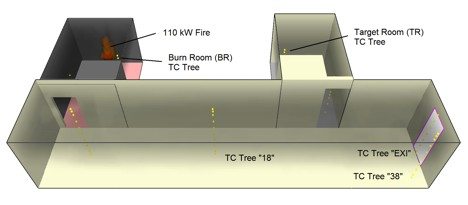
\includegraphics[width=5.0in]{FIGURES/NBS/NBS_Summary}\\
\end{center}
\caption{Overview of the NBS Test Configuration.}
 \label{fig:NBS_Summary}
\end{figure}

\begin{figure}[\figoptions{t}]
\begin{center}
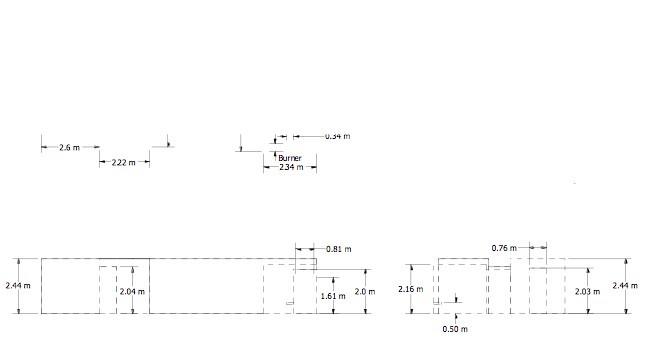
\includegraphics[width=8.0in, angle=90]{FIGURES/NBS/NBS_Detailed}\\
\end{center}
\caption{Plan, side and perspective schematic drawings of the NBS experimental arrangement, including the burner.}
 \label{fig:NBS_Detailed}
\end{figure}

Figures \ref{fig:NBS_HRR} show the experimentally measured $\dQ$ as a function of time during Tests 100A and 100Z, respectively, of the NBS multi-room test series, typically averaging about 100 kW.  In these two tests, for which the door was open, the $\dQ$ during the steady burning period measured via oxygen consumption calorimetry was about 110 kW $\pm$ 17 kW ($\pm$ 15 \%) \cite{NRCNUREG1824Experimental}. The combined relative expanded (2$\sigma$) uncertainty in the calorimetric  $\dQ$ is assigned a value of $\pm$~15~\%, consistent with the replicate measurements made during the experimental series and the uncertainty typical of oxygen consumption calorimetry \cite{NRCNUREG1824Experimental}. This value is also consistent with the measurement variation evident in the figures.  It was assumed that the closed door test (Test 100O) had the same $\dQ$ as the open door tests \cite{NRCNUREG1824Experimental}.

\begin{figure}[\figoptions{t}]
\begin{center}
\begin{tabular}{cc}
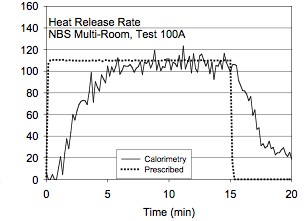
\includegraphics[width=3.0in]{FIGURES/NBS/NBS_HRR_100A} & 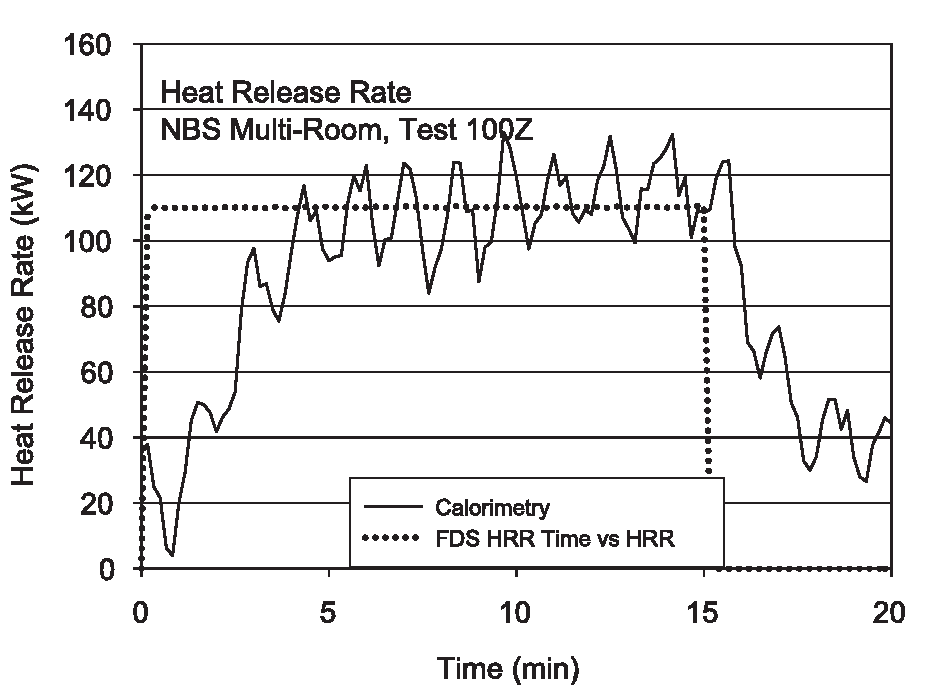
\includegraphics[width=3.0in]{FIGURES/NBS/NBS_HRR_100Z}\\
\end{tabular}
\end{center}
\caption{Prescribed and measured heat release rate as a function of time during Tests 100A and 100Z of the NBS multi-room test series.}
 \label{fig:NBS_HRR}
\end{figure}

The specified or prescribed  $\dQ$ is also shown in the figures.   The mass flow of the fuel (natural gas in Test 100A, or natural gas mixed with acetylene in Tests 100O and 100Z) was not metered; rather, the effluent was captured in a hood mounted above the open door in the corridor and the   was measured using oxygen consumption calorimetry.  The manner by which the fuel flow was controlled is not documented.  In Test 100A, candles were used to increase smoke in the upper layer to promote visualization. In Tests 100O and 100Z, acetylene was used (about 20 \% by volume) to produce smoke.  In those tests, the flow of natural gas and acetylene were adjusted to obtain approximately the same $\dQ$  as in Test 100A.  The addition of acetylene increased the radiative fraction of the fire. 

For practical reasons, piped natural gas supplied by large utility companies is often used in fire experiments.  While its composition may vary from day to day, there is little change expected in the value of the radiative fraction \cite{NRCNUREG1824Experimental}. As mentioned above, natural gas was used as the fuel in Test 100A.  In Tests 100O and 100Z, acetylene was added to the natural gas to increase the smoke yield, and as a consequence, the radiative fraction increased.  The radiative fraction of natural gas has been studied previously, whereas the radiative fraction of the acetylene/natural gas mixture has not been studied. The radiative fraction for the natural gas fire was assigned a value of 0.20, whereas a value of 0.30 was assigned for the natural gas/acetylene fires \cite{NRCNUREG1824Experimental, Hamins:1991}.  

The relative combined expanded (2$\sigma$) uncertainty in this parameter was assigned a value of $\pm$~20 \% in Test 100A and $\pm$~30 \% in 100O and 100Z.  The 20 \% expanded deviation value is consistent with typical values of the deviation reported in the literature for the measured radiative fraction.  The 100O and 100Z tests had a 50 \% larger value assigned, because the effect on the radiative fraction of adding acetylene to the natural gas was not measured \cite{NRCNUREG1824Experimental}.

Measurements made during the NBS test series included gas and surface temperature, pressure, smoke and major gas species concentration, and doorway gas velocity.  Only two types of measurements conducted during the NBS test series were used in the evaluation considered here, because there was less confidence in the other measurements.  The measurements considered here were the HGL temperature and depth, in which bare bead thermocouples were used to make these measurements.  Single point measurements of temperature within the burn room were not used in the evaluation of plume or ceiling jet algorithms.  This is because, in neither instance, was the geometry consistent with the assumptions used in the model algorithms of plumes or jets. Specifically, the burner was mounted against a wall, and the room width to height ratio was less than that assumed by the various ceiling jet correlations.

\section{FM Four Room Including Corridor Test Series}

This data set describes a series of tests conducted in a multiple room configuration with more complex gas burner fires than the previous data set.  This study \cite{Heskestad:1986} was included because, in many ways, it is similar to the smoke movement study performed at NBS \cite{Peacock:1988}, and permits comparisons between two different laboratories. In addition, it expands upon that data set by providing larger a time-varying gas burner fires in a room-corridor configuration. Fire size was about up to 1 MW with a total volume of 200 m$^3$.

This study was performed to collect data allowing for variations in fire source, ventilation, and geometry in a multi-compartment structure, especially for situations with closed doors. This test program was carried out at Factory Mutual Research Corporation (FMRC) in West Glocester, RI, in which 60 fire experiments were conducted in a multiple-room enclosure to furnish validation data for theoretical fire models.

Figure \ref{fig:FMSummary} shows a diagram of the basic facility with indications of instrumentation location. The facility was built on the floor of FMRC's fire test building, using part of the 67 m by 76 m test building where the ceiling height is 18.3 m. The layout in figure 25 shows a burn room and two target rooms connected to a corridor. The corridor was 2.43 m wide x 18.89 m long x 2.43 m high. The burn room measured 3.63 m deep x 3.64 m wide x 2.45 m high; a sealable window opening, measuring 0.85 m square, was centered on the rear wall, 0.34 m down from the top, and a door, measuring 0.92 m by 2.05 m high, was centered on the front wall (opening to the corridor). For closed window experiments, the wood-framed calcium silicate board window cover was pressed against a bead of caulking around the steel window frame and held by drop bars positioned into slots on the outside wall.

\begin{figure}[\figoptions{t}]
\begin{center}
\begin{tabular}{cc}
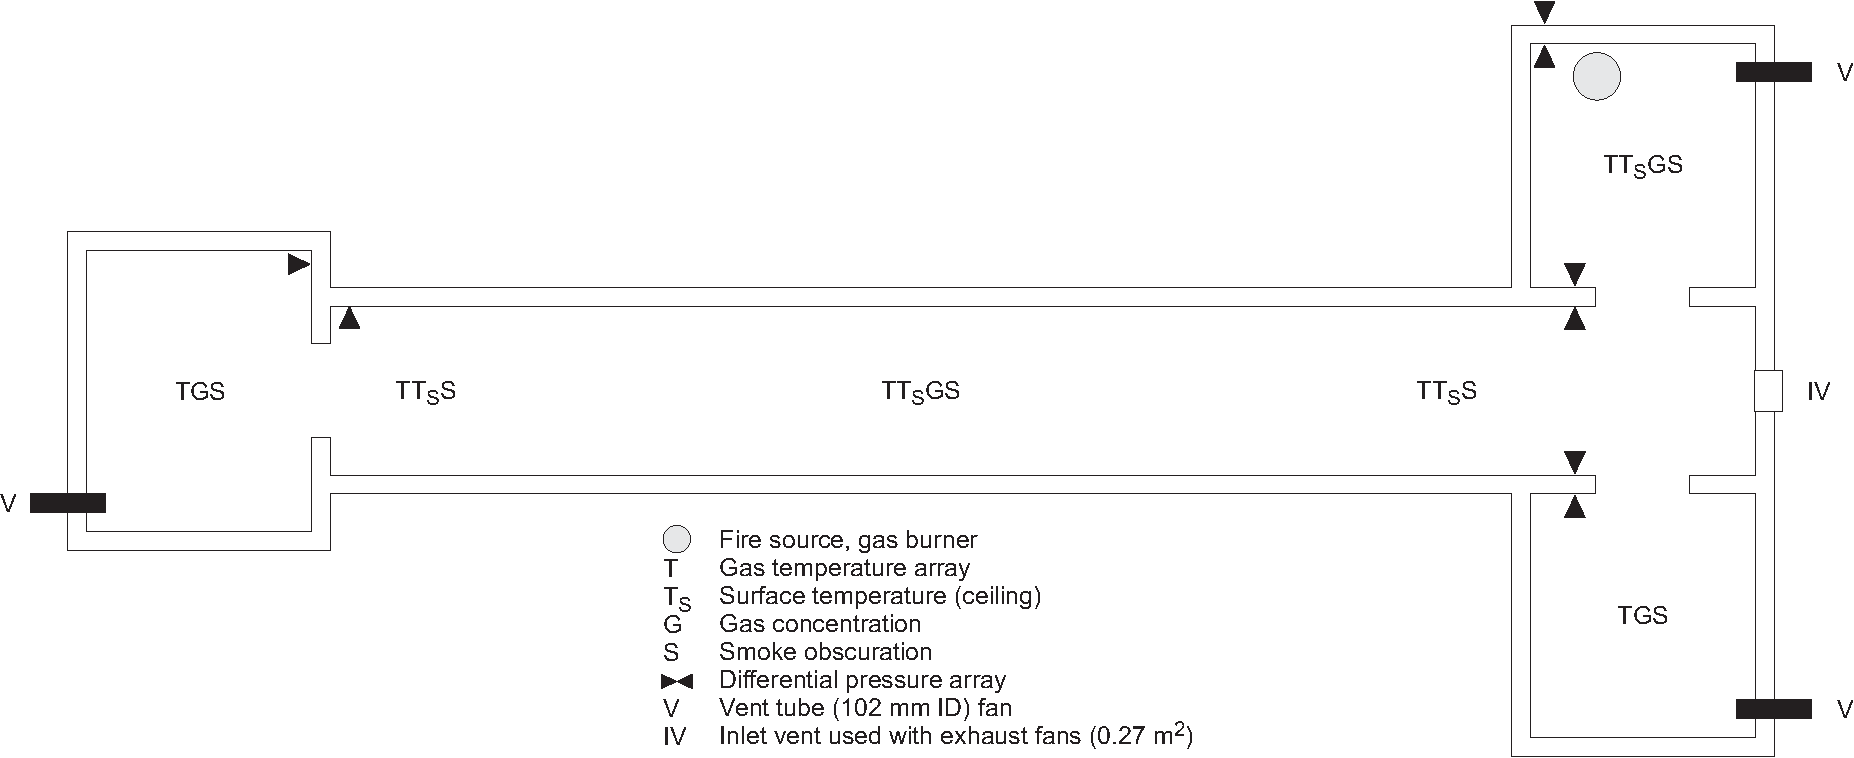
\includegraphics[width=6.0in]{FIGURES/FM/FMSummary}\\
\end{tabular}
\end{center}
\caption{Overview of the {F}actory {M}utual Four Room test series.}
 \label{fig:FMSummary}
\end{figure}

Room 3, located opposite the burn room, measured 3.65 m deep x 3.64 m wide x 2.45 in high; a door, measuring 0.88 m by 2.02 m high, was centered on the front wall (opening to the corridor). Room 4, located at the opposite end of the corridor, measured 3.65 m deep x 3.65 m wide x 2.43 m high and had a 0.88 m by 2.02 m high door centered on the front wall (opening to the corridor); an observation alcove, measuring 1.28 m by 0.86 m by 1.99 m high, was located in the front corner of room 4. Each room was equipped with a 102~mm inside diameter vent tube with a 61 mm inside diameter orifice meter and thermocouple, with option of exhaust fan (tube centered 0.27 m from the floor and 0.17 m from the closest parallel wall). An inlet vent (0.29 m$^2$) used with exhaust fans was centered 0.43 m above the floor at the end of the corridor between the burn room and room 3. When not in use, the inlet vent was sealed with a gypsum board cover taped in place.

The target room doors were commercial fire doors (wood-faced composite doors with calcium silicate cores, 14 h rated) mounted on 16 gage steel frames. The burn room door was fabricated from 12.7 mm calcium silicate, mounted in a steel frame lined with calcium silicate. Details of the doors and the spacings (cracks) are given in the original reference \cite{Heskestad:1986}. 

Gypsum wallboard, 12.7 mm thick, on wood studs was used throughout the experimental facility. In addition, the walls and ceiling of the burn room were overlaid with calcium silicate, also 12.7 mm thick, to harden against repeated fire exposure. The existing concrete floor of the test building was used.

Two types of fire sources were used: 1) steady propylene fires at 56 kW on a 0.30 m diameter sand burner and 522 kW on a 0.91 m diameter burner and 2) propylene fires on the 0.91 m diameter burner programmed under computer control to grow with the square of time, exceeding 1 MW in 1, 2, 4, or 8 min.

The 0.91 m diameter, 0.58 in high propylene burner was used for most of the tests. Its design consisted of a 12 gage steel container with a gas distributor near the bottom, filled with gravel to a 67 percent height, where there was wire mesh screen, and coarse sand to the full height of the burner. The 0.30 m diameter burner was a scaled-down version of similar design.

\section {NIST Seven-story Hotel Tests}

By far the most complex test, this data set is part of  a series of full-scale experiments conducted to evaluate zoned smoke control systems, with and without stairwell pressurization \cite{Klote:1990}.  It was conducted in a seven story hotel with multiple rooms on each floor and a stairwell connecting all floors.  This data set was chosen because it would challenge the scope of most current fire models.  Measured temperatures and pressure differences between the rooms and floors of the building are extensive and consistent.  Peak fire size was 3 MW with a total building volume of 140~000 m$^3$.

Smoke movement and the performance of smoke control systems were studied in a seven story hotel building with smoke generated from wood fires and theatrical smoke. A total of 12 single experiments
were conducted under a variety of conditions: two different fire sizes; sprinklered vs non-sprinklered wood fires; zoned smoke control on or off; stairwell pressurization on or off; with and without ventilation to the outside; and open and closed doors. 

The Plaza Hotel building was a masonry structure consisting of two wings, one three stories and the other seven stories tall. The two wings were built at different times. The wings were connected to each other at only one location on each floor. The connections between the wings at each floor were sealed off, and the fires were set on the second floor of the seven-story wing, using the shorter wing as an instrumentation area. Areas of the second floor were fire hardened to minimize structural damage to the building.

\begin{figure}[\figoptions{t}]
\begin{center}
\begin{tabular}{cc}
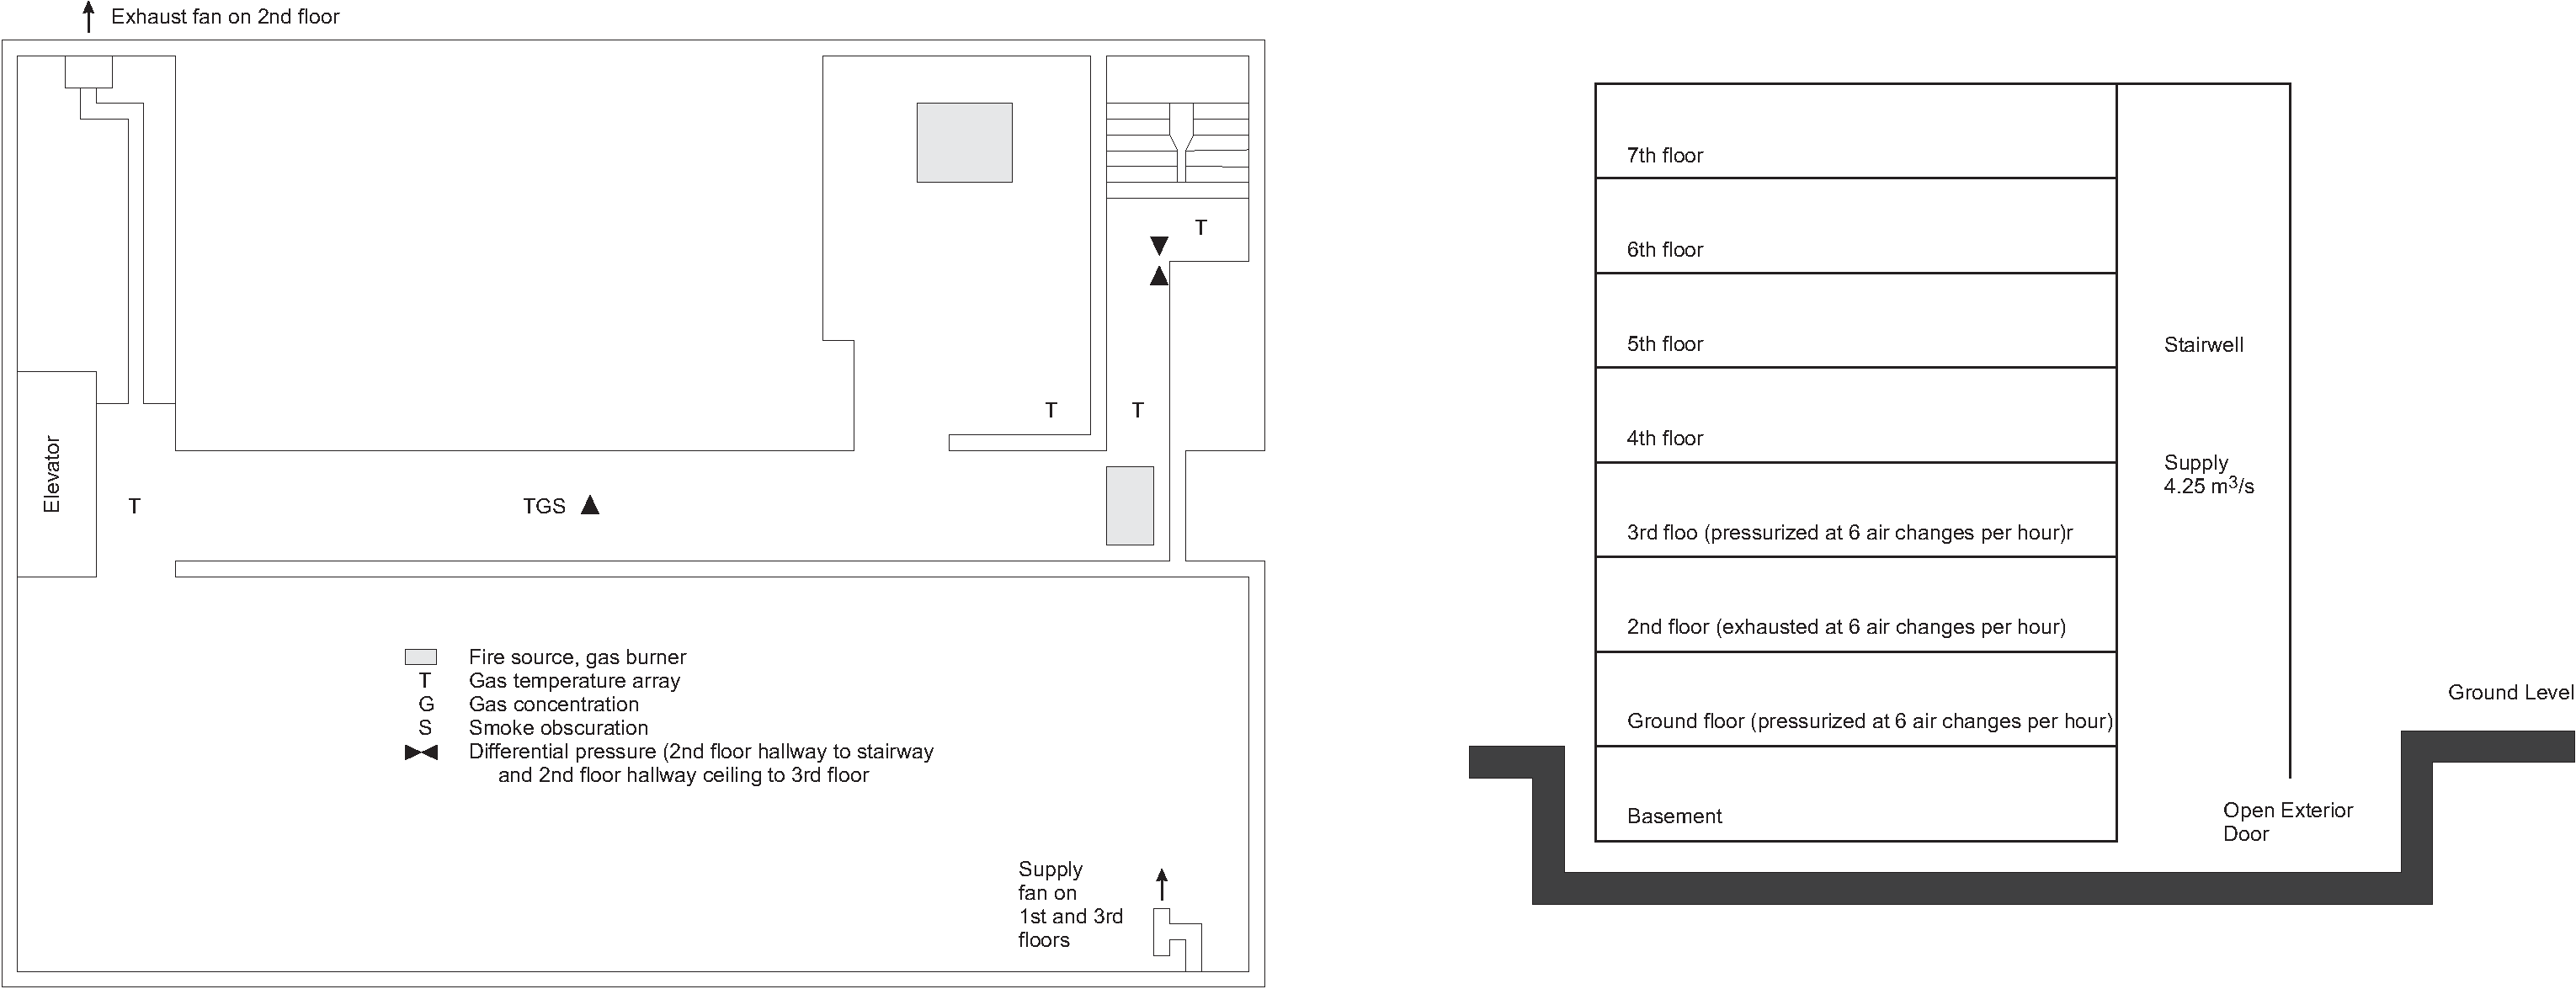
\includegraphics[width=6.0in]{FIGURES/NIST_PLAZA/PlazaSummary}\\
\end{tabular}
\end{center}
\caption{Overview of the NIST Seven-story hotel test series including smoke control.}
 \label{fig:PlazaSummary}
\end{figure}

The smoke control systems were designed using the methods presented in the ASHRAE smoke control manual \cite{Klote:1983}, and the design analysis is discussed in detail by Klote \cite{Klote:1988}. The minimum design pressure difference was 25 Pa, meaning that the system should be able to maintain at least this value without a fire. The Plaza Hotel building had no central forced air heating, ventilating, and air-conditioning (HVAC) system, so a dedicated system of fans and ducts was installed for zoned smoke control and stairwell pressurization. The smoke control system consisted of the three 0.944 m$^3$/s centrifugal fans shown in \ref{fig:PlazaSummary}, plus another centrifugal fan (not shown) located outside and supplying 4.25 m$^3$/s of pressurization air to the stairwell at the first floor. The smoke control system is illustrated in figure \ref{fig:PlazaSummary}. All the test fires were located in the second floor smoke zone. This smoke was exhausted at about six air changes per hour. The first and second floors were pressurized at about six air changes per hour. When the stairwell pressurization system was activated, the exterior stairwell door was open. This approach is intended to minimize fluctuations due to opening and closing doors.



